\documentclass[8pt,landscape]{article}
\usepackage{multicol}
\usepackage{calc}
\usepackage{hyperref}
\usepackage{amsmath, amsthm, amssymb,graphicx,rcs,datetime,qtree,moreverb, , tikz}
\usepackage{algorithm}				% This package is for algorithms
\usepackage[noend]{algpseudocode}   
\usepackage{ifthen}
\usepackage[landscape]{geometry}
\usepackage{amsmath,amsthm,amsfonts,amssymb}
\usepackage{color,graphicx,overpic}
\usepackage{latexsym}
\usepackage{hyperref}
\usepackage{listings}
\usepackage[normalem]{ulem}
\usepackage{esvect}
\lstset{
  basicstyle=\ttfamily,
  columns=fullflexible,
  frame=single,
  breaklines=true,
  postbreak=\mbox{\textcolor{red}{$\hookrightarrow$}\space},
}

\pdfinfo{
  /Title (midterm.pdf)
  /Creator (TeX)
  /Producer (pdfTeX 1.40.0)
  /Author (Kieran)
  /Keywords (pdflatex, latex,pdftex,tex)}

% This sets page margins to .5 inch if using letter paper, and to 1cm
% if using A4 paper. (This probably isn't strictly necessary.)
% If using another size paper, use default 1cm margins.
\ifthenelse{\lengthtest { \paperwidth = 11in}}
    { \geometry{top=.1in,left=.1in,right=.1in,bottom=.1in} }
    {\ifthenelse{ \lengthtest{ \paperwidth = 297mm}}
        {\geometry{top=1cm,left=1cm,right=1cm,bottom=1cm} }
        {\geometry{top=1cm,left=1cm,right=1cm,bottom=1cm} }
    }

% Turn off header and footer
\pagestyle{empty}

% Redefine section commands to use less space
\makeatletter
\renewcommand{\section}{\@startsection{section}{1}{0mm}%
                                {-1ex plus -.5ex minus -.2ex}%
                                {0.5ex plus .2ex}%x
                                {\normalfont\large\bfseries}}
\renewcommand{\subsection}{\@startsection{subsection}{2}{0mm}%
                                {-1explus -.5ex minus -.2ex}%
                                {0.5ex plus .2ex}%
                                {\normalfont\normalsize\bfseries}}
\renewcommand{\subsubsection}{\@startsection{subsubsection}{3}{0mm}%
                                {-1ex plus -.5ex minus -.2ex}%
                                {1ex plus .2ex}%
                                {\normalfont\small\bfseries}}
\makeatother

% Define BibTeX command
\def\BibTeX{{\rm B\kern-.05em{\sc i\kern-.025em b}\kern-.08em
    T\kern-.1667em\lower.7ex\hbox{E}\kern-.125emX}}

% Don't print section numbers
\setcounter{secnumdepth}{0}


\setlength{\parindent}{0pt}
\setlength{\parskip}{0pt plus 0.5ex}

%My Environments
\newtheorem{example}[section]{Example}
% -----------------------------------------------------------------------

\begin{document}
\raggedright
\scriptsize
\begin{multicols}{3}


% multicol parameters
% These lengths are set only within the two main columns
%\setlength{\columnseprule}{0.15pt}
\setlength{\premulticols}{1pt}
\setlength{\postmulticols}{1pt}
\setlength{\multicolsep}{1pt}
\setlength{\columnsep}{2pt}

\begin{center}
     \Large{\underline{3GC3 - Kieran Henderson}} \\
\end{center}

\section{Pref quals for high quality triangle mesh}
- Close to EQUILATERAL triangles
- Vertex close to 6$^{\circ}$
- Angles close to 60$^{\circ}$

\section{Manifolds}
- Every edge is shared by exactly 2 triangles
- There is a single complete loop of triangles around each vertex

\section{Manifolds with Boundary}
- Every edge is shared by 1 or 2 triangles 
- Vertex connect to a single edge connected triangle loop (can not connect 2 different groups of triangles)
- Every manifold is also a manifold with boundary

\section{Texture Wrapping}
GL\_CLMAP\_TO\_EDGE = take outer most pixels and repeat until the edge is reached\\
GL\_REPEAT = repeat the image in a grid with all oriented the same way\\
GL\_MIRRORED\_REPEAT = repeat image in a grid with all mirrored along axis between original and new\\

\section{Barycentric interpolation of texture coords}
Ex. For texture position (0.5, 0.4, 0)\\
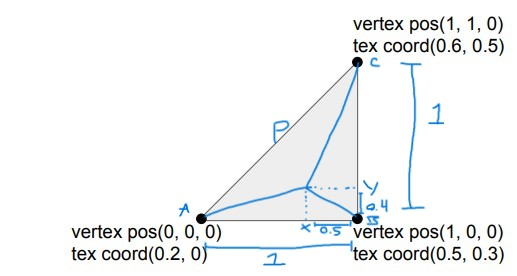
\includegraphics[width=0.2\textwidth]{bary.jpg}
$S_{ABC} = \frac{AB * AC}{2} = \frac{1 * 1}{2} = 0.5$\\
$S_{PAB} = \frac{AB * PX}{2} =\frac{1 * 0.4}{2} = 0.2$\\
$S_{PBC} = \frac{BC * PY}{2} = \frac{1 * 0.5}{2} = 0.25$\\
So $P = \alpha A + \beta B + \gamma C$ Where $\alpha, \beta, \gamma$ are the barycentric coords of P\\
$\alpha = \frac{S_{PBC}}{S_{ABC}} = \frac{0.25}{0.5} = 0.5$\\
$\gamma = \frac{S_{PAB}}{S_{ABC}} = \frac{0.2}{0.5} = 0.4$\\
$\beta = 1 - \alpha - \gamma = 1 - 0.5 - 0.4 = 0.1$\\
So $P = 0.5 A + 0.1 B + 0.4 C$\\$ = 0.5(0.2, 0) + 0.1(0.5,0.3) + 0.4(0.6,0.5)$\\$ = (0.1, 0) + (0.05,0.03) + (0.24,0.2)$ \\ $ = (0.39,0.23)$\\

\section{Bilinear texture filtering}
Ex. For vertex v's texture coord (0.2, 0.3)\\
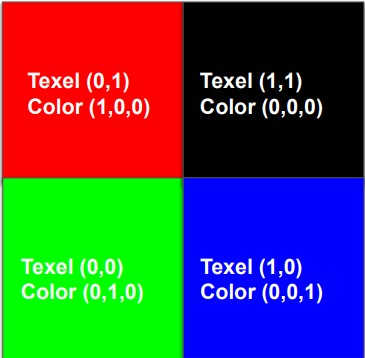
\includegraphics[width=0.2\textwidth]{textCoord.jpg}
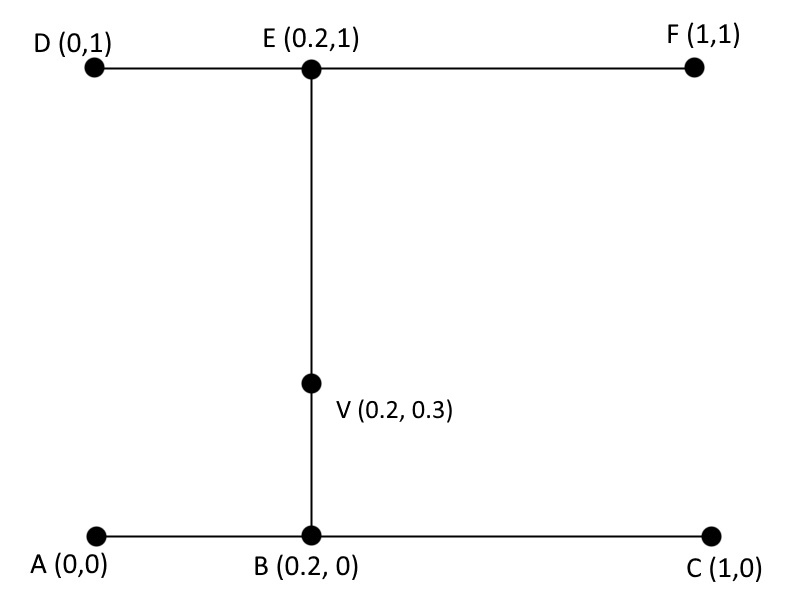
\includegraphics[width=0.2\textwidth]{texChart.jpg}

Color of E:\\
$ E = 0.8C + 0.2D = 0.8(1,0,0) + 0.2(0,0,0) = (0.8, 0, 0)$\\
Color of B:\\
$B = 0.8A + 0.2C = 0.8(0,1,0) + 0.2(0,0,1) = (0, 0.8, 0.2)$\\
Color of V:\\
$V = 0.7B + 0.3E = 0.7(0,0.8,0.2) + 0.3(0.8,0,0) = (0.24,0.56,0.14)$\\

\section{Level of mipmap}
mipmap level = $log_2 D$ where D = length of longest edge\\
Just approximate the size of the longest edge and use calculator $log_2(x) =  log(x) / log(2)$\\

\section{Types of maps}
Nothing:\\
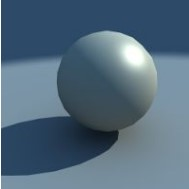
\includegraphics[width=0.1\textwidth]{dis1.jpg}

Displacment map:\\
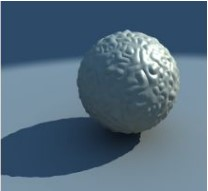
\includegraphics[width=0.1\textwidth]{dis2.jpg}

Bump map:\\
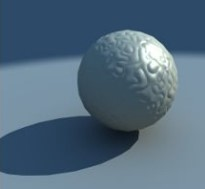
\includegraphics[width=0.1\textwidth]{dis3.jpg}

\section{Properties of light sources}
Point Light - Illuminate in all directions and attenuated with distance\\
Directional Light - The light rays are nearly parallel to each other and there is no attenuation with distance\\
Spot Light - illuminates in a specific direction and attenuated with distance\\
Ambient Light - Tries to approximate global illuination and has a constant irradiance at every location and in all directions\\

\section{Specular Exponent} 
Smaller specular exponent = larger shiny/white area\\
Larger specular exponent = smaller shiny/white area\\ 

\section{Properties of Curves}
Single Polynomial - Interpolation, $C^2$ continuity, \sout{Locality}\\
Natual Cubic Spline - Interpolation, $C^2$ continuity, \sout{Locality}\\
Hermite Cubic Spline - Interpolation, \sout{$C^2$ continuity} $C^1$, Locality\\
Vardinal/Catmull-Rom - Interpolation, \sout{$C^2$ continuity} $C^1$, Locality\\

\section{Hermite vs Vardinal cubic Splines}
Hermite - Users have to specify first derivatives of all control points\\
Cardinal - First derivatives are calculated from the neighbor control points\\

\section{Terminology}
Radiant Flux $\Phi$ - Power with units in W or J/s\\
Irradiance E - Power per unit area with unit in $\frac{W}{m^2}$\\
Radiance L - Power per unit area per direction with unit in $\frac{W}{m^2*sr}$\\
Radiant Intensity I - Power per direction with unit in $\frac{W}{sr}$\\

\section{Acronyms}
BRDF - Bidirectional Reflectance Distribution Function\\
AABB - Axis-Aligned Bounding Box\\
BVH - Bounding Volume Hierachy\\
BSP - Binary Space Partition\\

\section{Hemisphere Projection}
Object has area S=100, and it is projected onto hemisphere with radius r=3, the projected area is A=45. What is the solid angle of this object with respect to the point p?\\
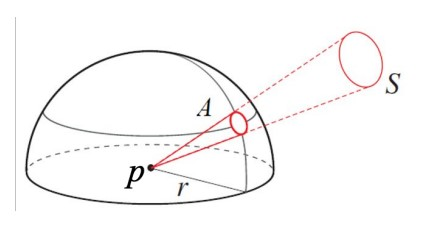
\includegraphics[width=0.2\textwidth]{proj.jpg}
solid angle $= \frac{A}{r^2} = \frac{45}{9} = 5$\\

\section{Rendering Equation}
$L(P,\omega_o) = L_e(P,\omega_o) + \int_{\Omega} f_r(P, \omega_i,\omega_o) L_i(P,\omega_i)cos\Theta_idw_i$\\
$L_e$ = emiting light radiance\\
$f_r$ = reflection of incoming light\\
$\omega_i$ = incoming direction\\
$\omega_o$ = outcoming direction\\
$L_i$ = incoming light radiance\\

\section{Reflection models}
Phong - Uses the angle between the view and reflection vector for computing specular reflection\\
Blinn-Phong - Uses the angle between the normal and halfway vector for computing specular reflection\\

\section{Shading models}
Gouraud - Uses pervertex color computation\\
Phong - Uses perfragment color computation\\

\section{Mirrored reflection calculation}
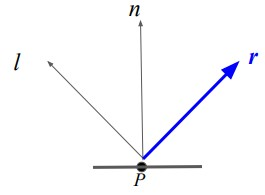
\includegraphics[width=0.2\textwidth]{ref.jpg}\\
$\vec{r}^{\,} = - \vec{l}^{\,} + 2(\vec{l}^{\,} * \vec{n}^{\,}) \vec{n}^{\,}$

\section{Ray tracing Modes}
Perspective:\\
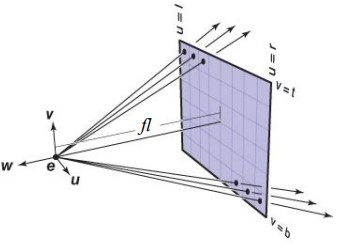
\includegraphics[width=0.2\textwidth]{persp.jpg}\\
Orthographic:\\
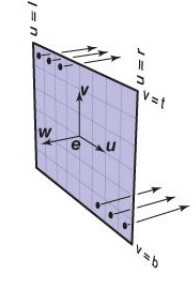
\includegraphics[width=0.2\textwidth]{orth.jpg}\\

\section{Raytracing Calculation}
Ray r = o + t d, where o(2,3,4), d(-1, 0, 0), what is the t value when it intersects with plane y=3x?\\
$r = o + td = (2,3,4) + t(-1,0,0) = (2-t,3,4)$\\
$y = 3x \rightarrow 3 = 3 (2-t) \rightarrow y/3 = 2-t \rightarrow 1 = 2-t \rightarrow t = 1$\\

\section{Data structures}
Quad-tree:\\
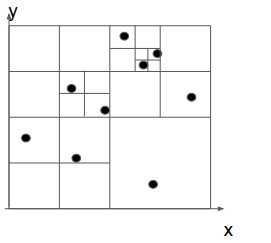
\includegraphics[width=0.2\textwidth]{quad.jpg}\\
BVH:\\
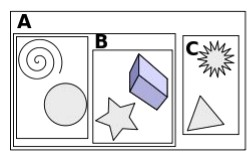
\includegraphics[width=0.2\textwidth]{bvh.jpg}\\
BSP:\\
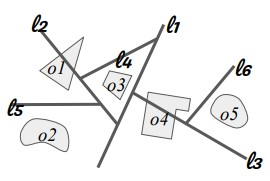
\includegraphics[width=0.2\textwidth]{bsp.jpg}\\
KD tree:\\
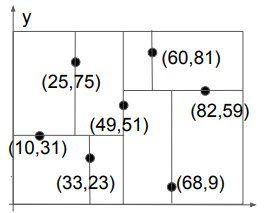
\includegraphics[width=0.2\textwidth]{ko.jpg}\\

\section{Data structure Applications}
Quad - Image Compression\\
BVH - Ray Tracing\\
BSP - Painter's Algo\\
KD tree - Nearest Neighbor Search\\

\section{Triangle Mesh Representation}
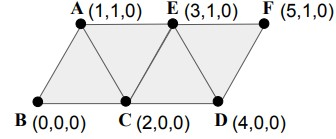
\includegraphics[width=0.2\textwidth]{mesh.jpg}\\
vertices = [(1, 1, 0), (0, 0, 0), (2, 0, 0), (4, 0, 0), (3, 1, 0), (5, 1, 0)]\\
triangles = [(0, 1, 2), (0, 2, 4), (4, 2, 3), (4, 3, 5)]\\



% You can even have references
\scriptsize
\end{multicols}
\end{document}